Efficiencies of muons are measured using the same method used for electron measurements i.e. Tag-and-Probe (TnP) method performed on
$Z \to \Pgm\Pgm$ and $ \jpsi\to\mu\mu$ events in bins of $\pt$ and $\eta$. More
details on the methodology are described in Section. \ref{tnp_procedure} and also in Ref.~\cite{CMS_AN_2015-277}. Measurements are extracted using 2018 RunA,B,C,D data while the measurements corresponding to 2016 and 2017 datasets have already been reported in Ref.~\cite{CMS_AN_2016-442} and Ref.~\cite{CMS_AN_2017-342} respectively.
%
For the measurement of muon reconstruction and identification efficiency at high $\pt$ ($\pt$>20 GeV), and impact parameter requirements and isolation efficiencies for all $\pt$, $\Z$ sample is used.  to measure the muon reconstruction and identification efficiency at high $\pt$,
and the efficiency of the isolation and impact parameter requirements at all $\pt$.
%
To measure the reconstruction and identification efficiency at low $\pt$, $\jpsi$ sample is used as it benefits from a better purity in that kinematic regime. In this case,
events are collected using \verb=HLT_Mu7p5_Track2_Jpsi_v*= when probing the
reconstruction and identification efficiency in the muon system, and using the
 \verb=HLT_Mu7p5_L2Mu2_Jpsi_v*= when probing the tracking efficiency.

\paragraph*{Muon reconstruction and identification efficiency measurement}

Results for muon reconstruction and identification efficiencies for high $\pt$ muons ($\pt>20\GeV$) have been derived by the Muon POG.
The probe in this measurement are tracks of inner tracker, and
the passing probes are those which are also regarded as a global or tracker muon 
and passing the Muon POG Loose muon identification.
%
Results for low~\pt~ muons were derived using \Jpsi events, with the same definitions
of probe and passing probes. The systematic uncertainties on the measurements are estimated by including several variations e.g. varying the analytical signal and background shape models used to fit distribution of dimuon invariant mass. Furthermore, number of bins in dimuon distribution and mass window are also increased and decreased to include systematic effects. Details on the procedure can be found in Ref.~\cite{AN-15-277}. The efficiency and scale 
factors used for low $\pt$ muons are the ones derived using single muon prompt-reco dataset.

The data and simulation efficiencies and their ratios in bins are shown in Figure ~\ref{fig:MuonIDEff_1}. 
\begin{figure}[htbp]
  \begin{center}
    \subfigure[]{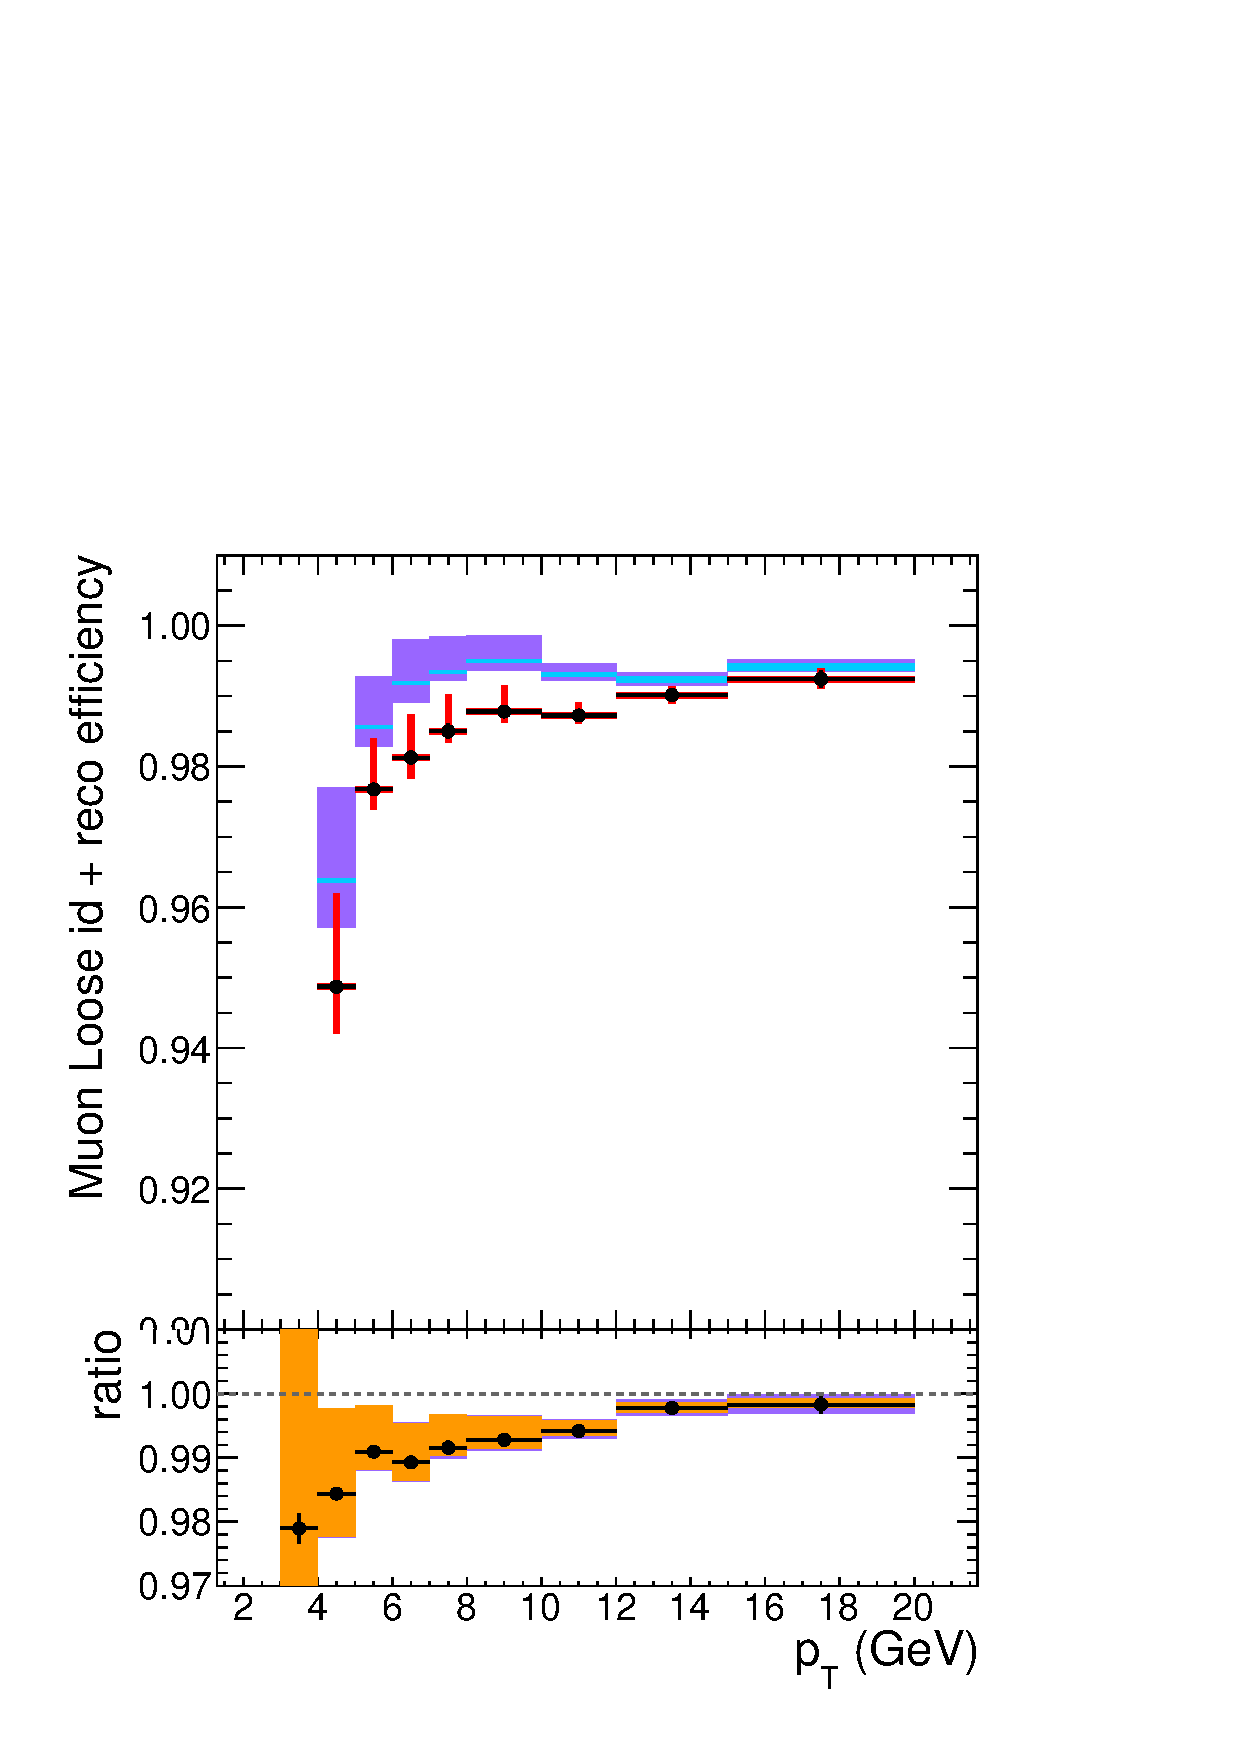
\includegraphics[width=0.32\textwidth]{Figures/Muons/mu_Loose_barrel.pdf}}
    \subfigure[]{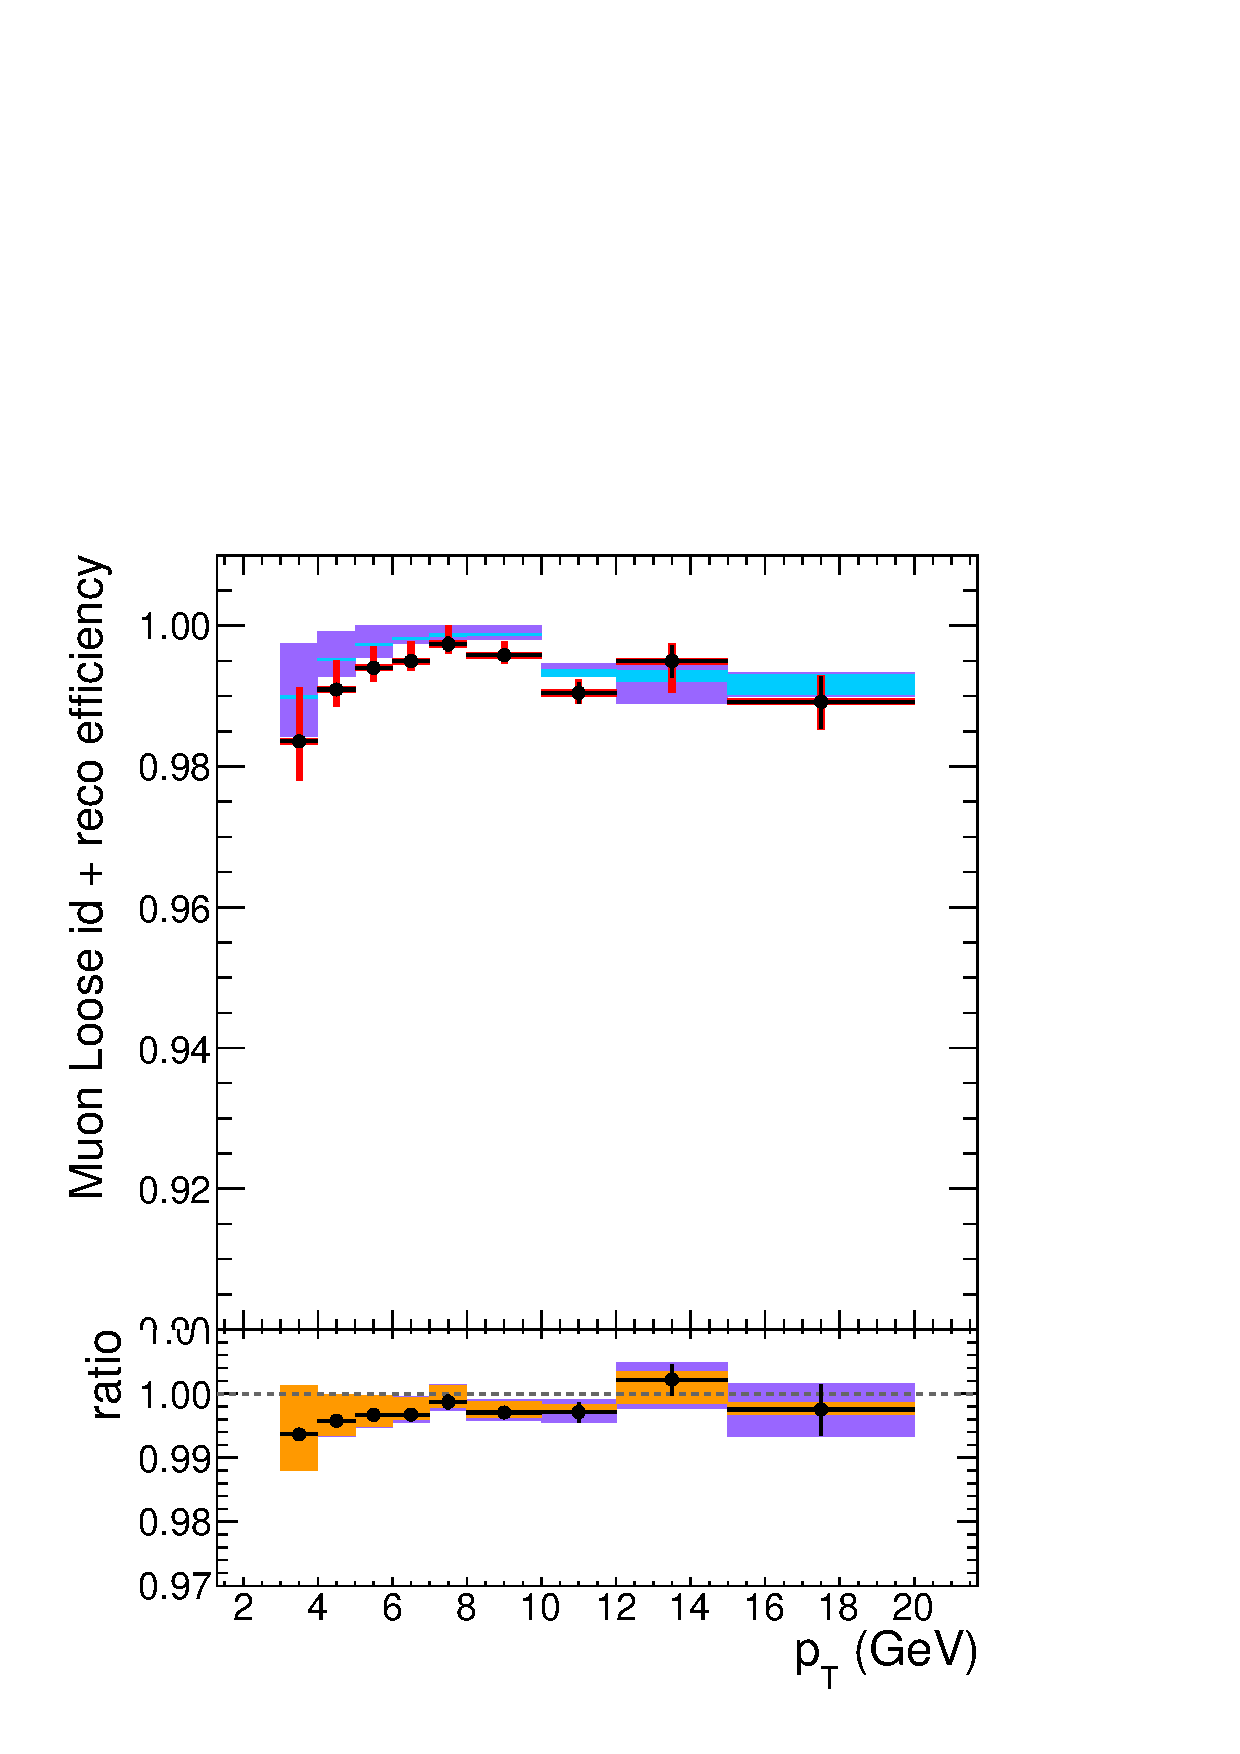
\includegraphics[width=0.32\textwidth]{Figures/Muons/mu_Loose_endcap.pdf}}
    \subfigure[]{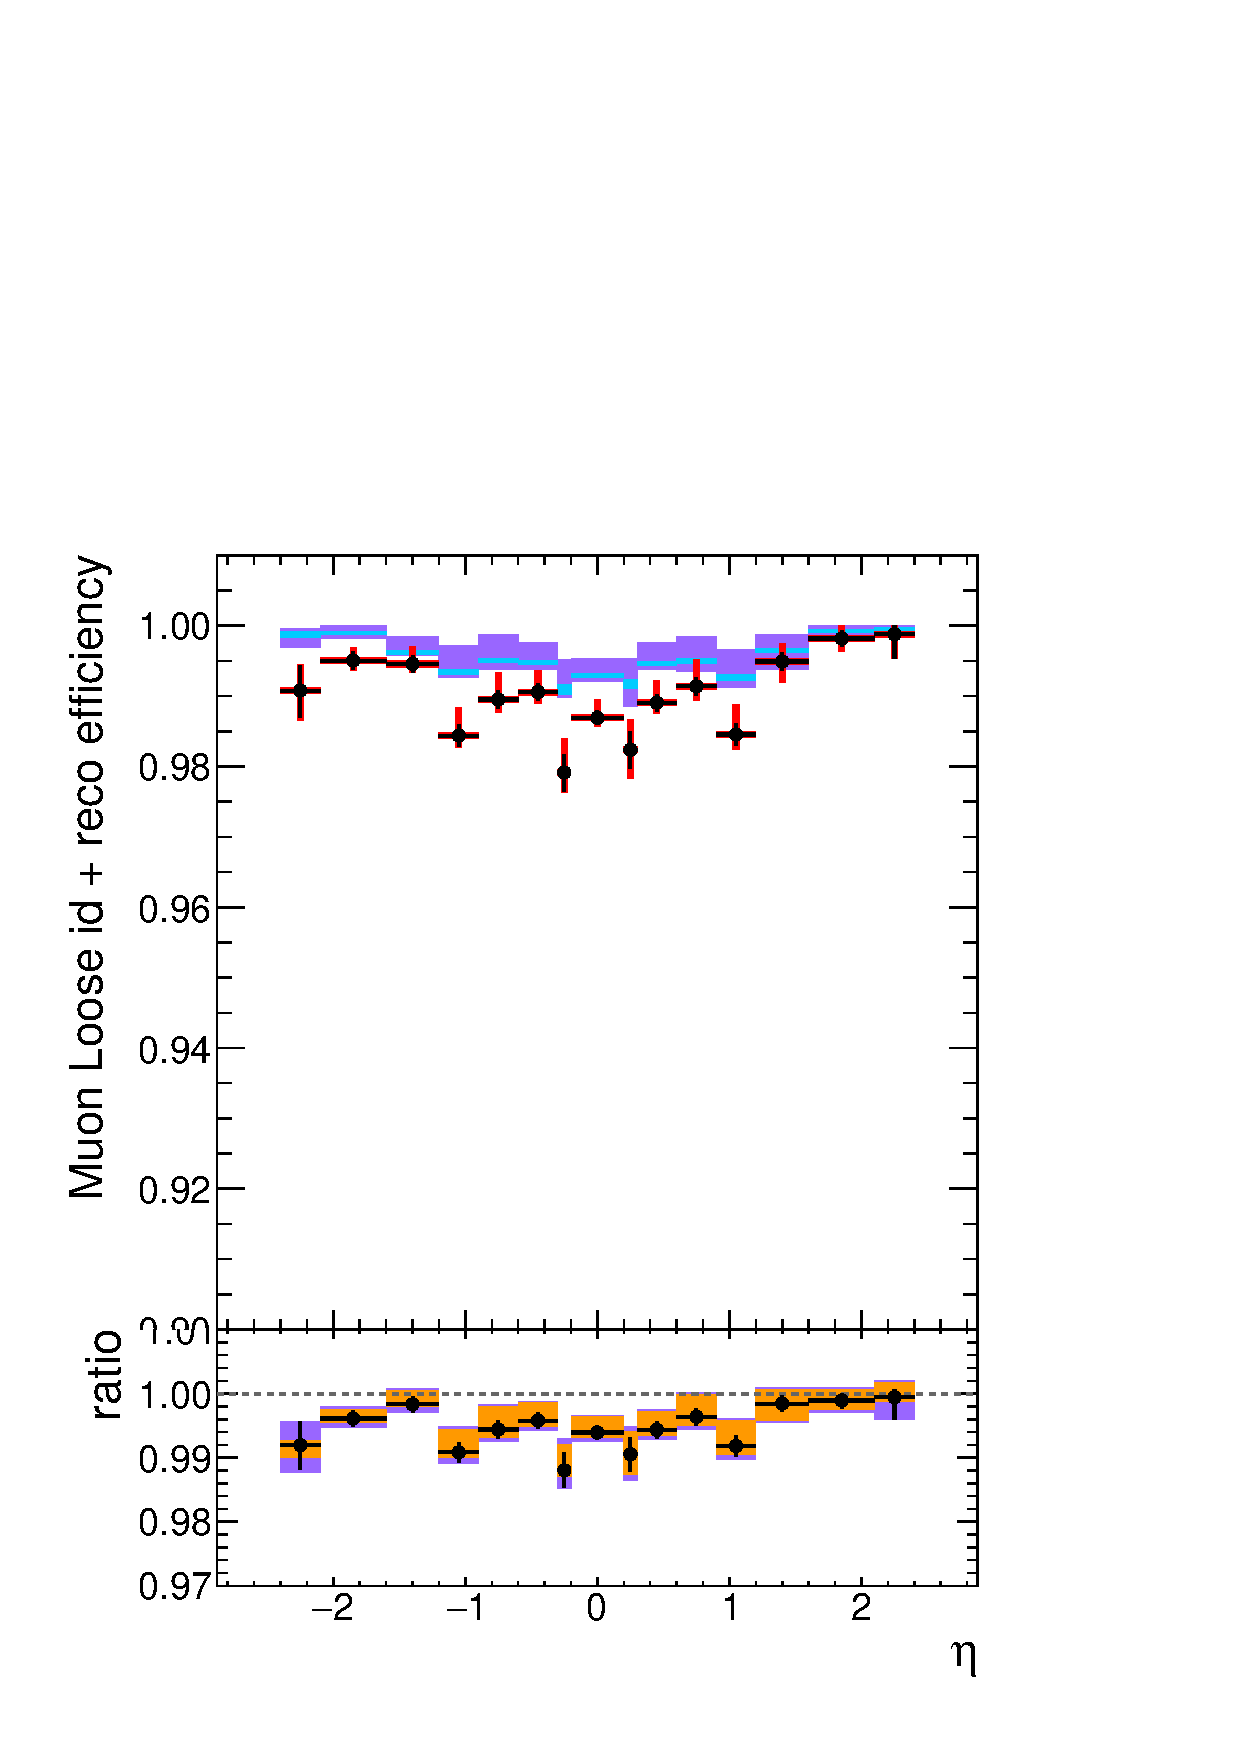
\includegraphics[width=0.32\textwidth]{Figures/Muons/mu_Loose_pt7.pdf}}
    \caption{Reconstruction and identification efficiencies of muons at low \pt, measured with the $TnP$ method on \Jpsi events, in bins of~\pt~ in barrel (left) and endcaps (center), and in terms of $\eta$ for $\pt > 7\GeV$ (right). In upper panel of each diagram, the larger uncertainty bars include also the systematical uncertainties, while the smaller ones are purely statistical. In the lower panel showing the ratio of two efficiencies, black uncertainty bars are for statistical uncertainty, the orange rectangles for the systematical uncertainty and the violet rectangles include both uncertainties.}
    \label{fig:MuonIDEff_1}
\end{center}
\end{figure}

\paragraph*{Efficiency measurement of muon impact parameter requirement}
The measurement is performed using $\Z$ events. Events are selected with \verb=HLT_IsoMu27_v*= or \verb=HLT_Mu50_v*= triggers.
For this measurement, the probe is a muon passing the POG Loose identification criteria,
and it is considered a passing probe if satisfies the SIP3D, dxy, dz cuts of this analysis.
%
The results are shown in the Figure ~\ref{fig:MuonIDEff_2}.
%Very good agreement between data and simulation is observed in the barrel (Fig.~\ref{fig:MuonIDEff_2}, left)
%while some inefficiency is visible in the endcaps, especially at large values of $|\eta|$.
%The data to simulation scale factor is found to be flat as function of \pt, so, similarly to what done
%for the identification part, we apply a correction only as function of $\eta$.
\begin{figure}[htbp]
  \begin{center}
    \subfigure[]{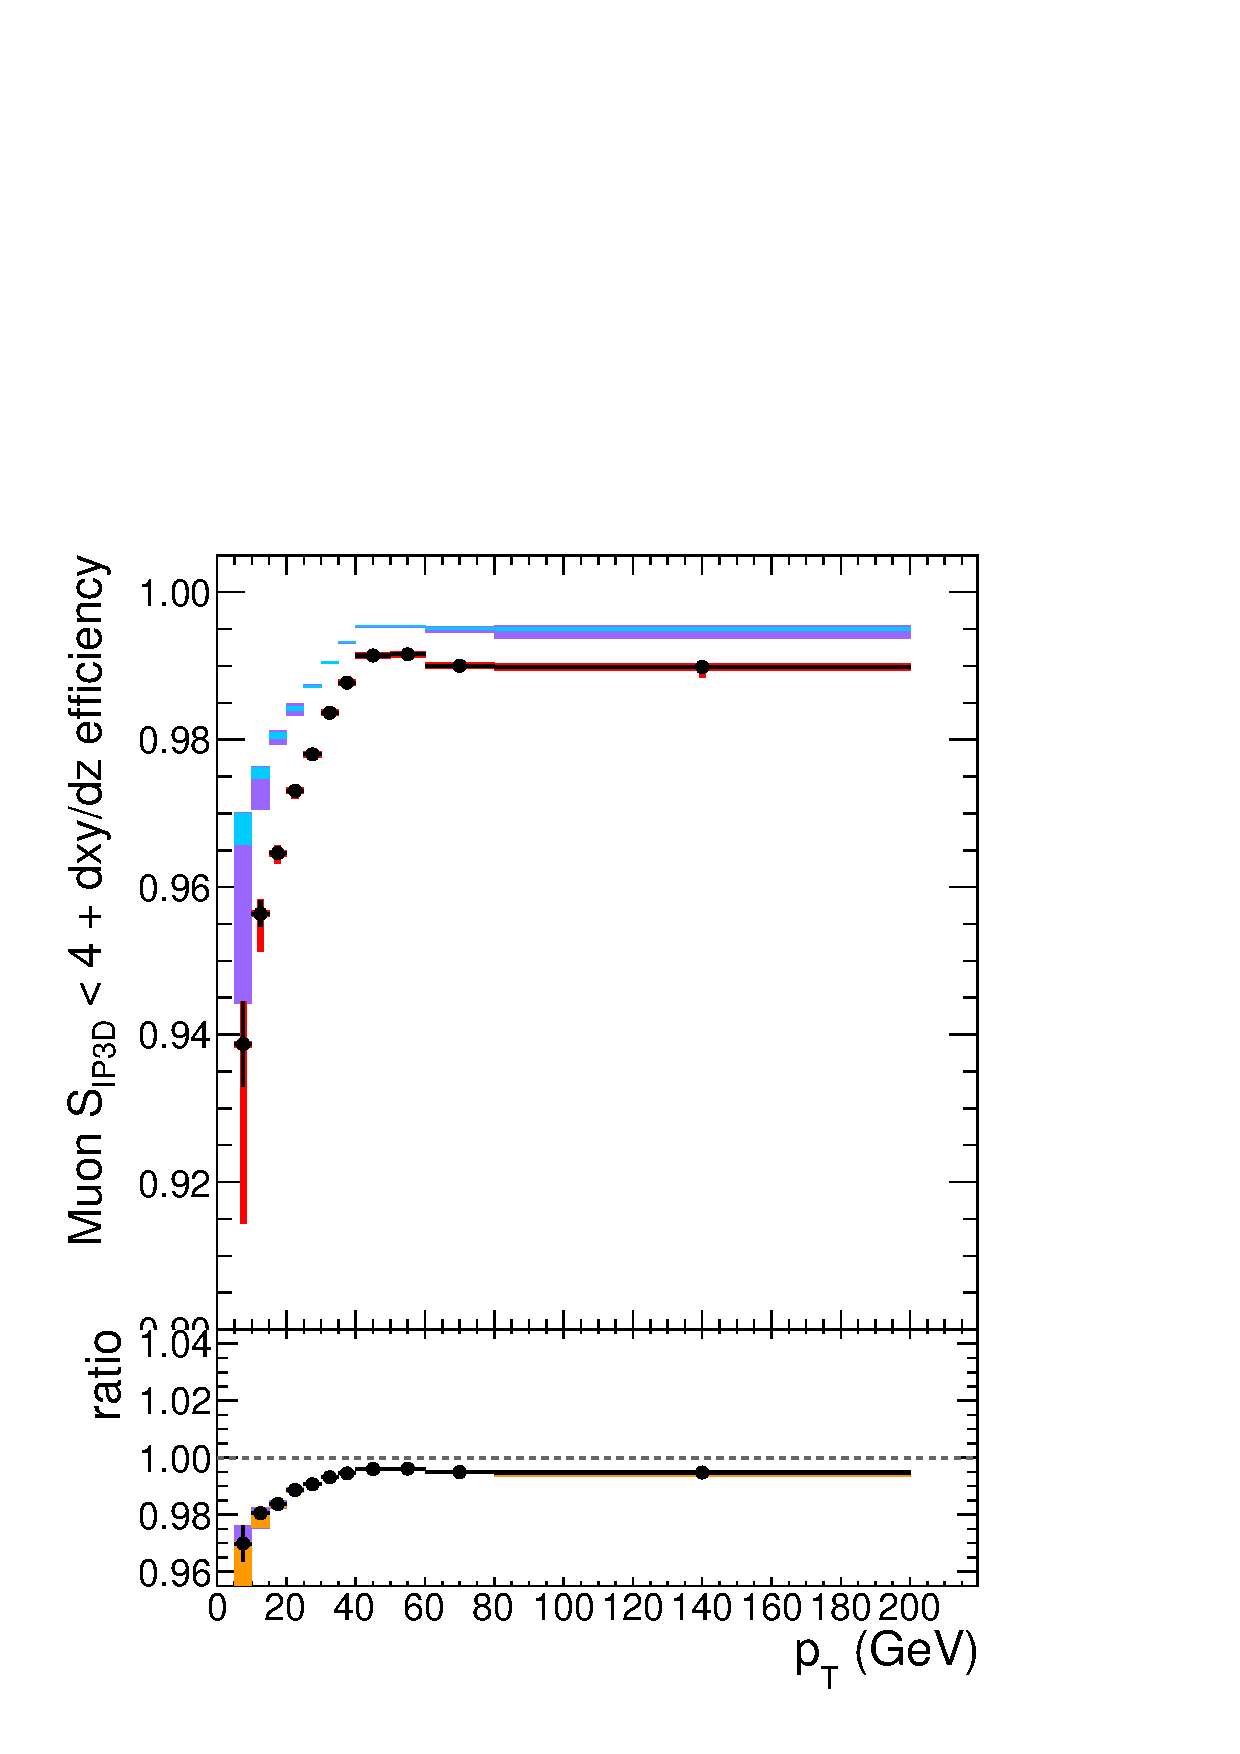
\includegraphics[width=0.32\textwidth]{Figures/Muons/mu_SIP4_barrel.pdf}}
    \subfigure[]{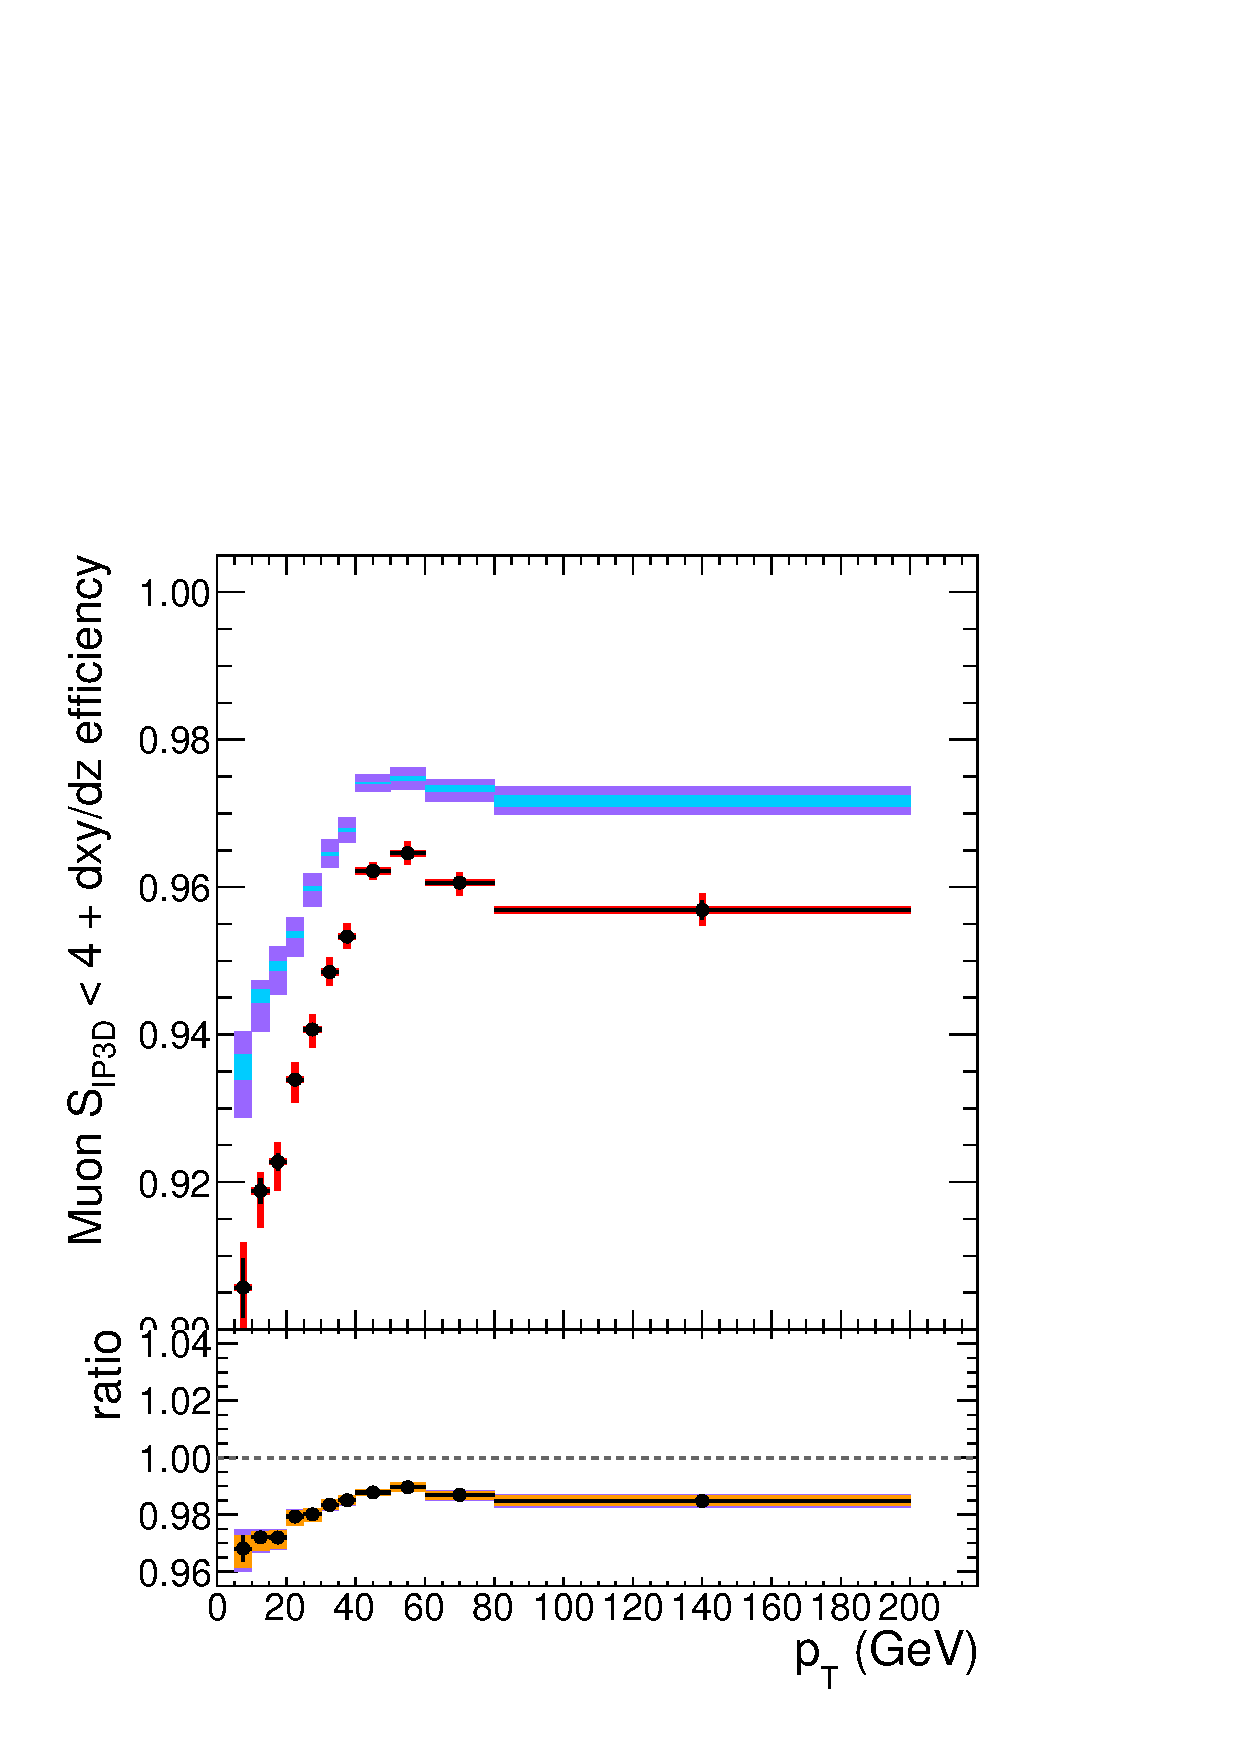
\includegraphics[width=0.32\textwidth]{Figures/Muons/mu_SIP4_endcap.pdf}}
    \subfigure[]{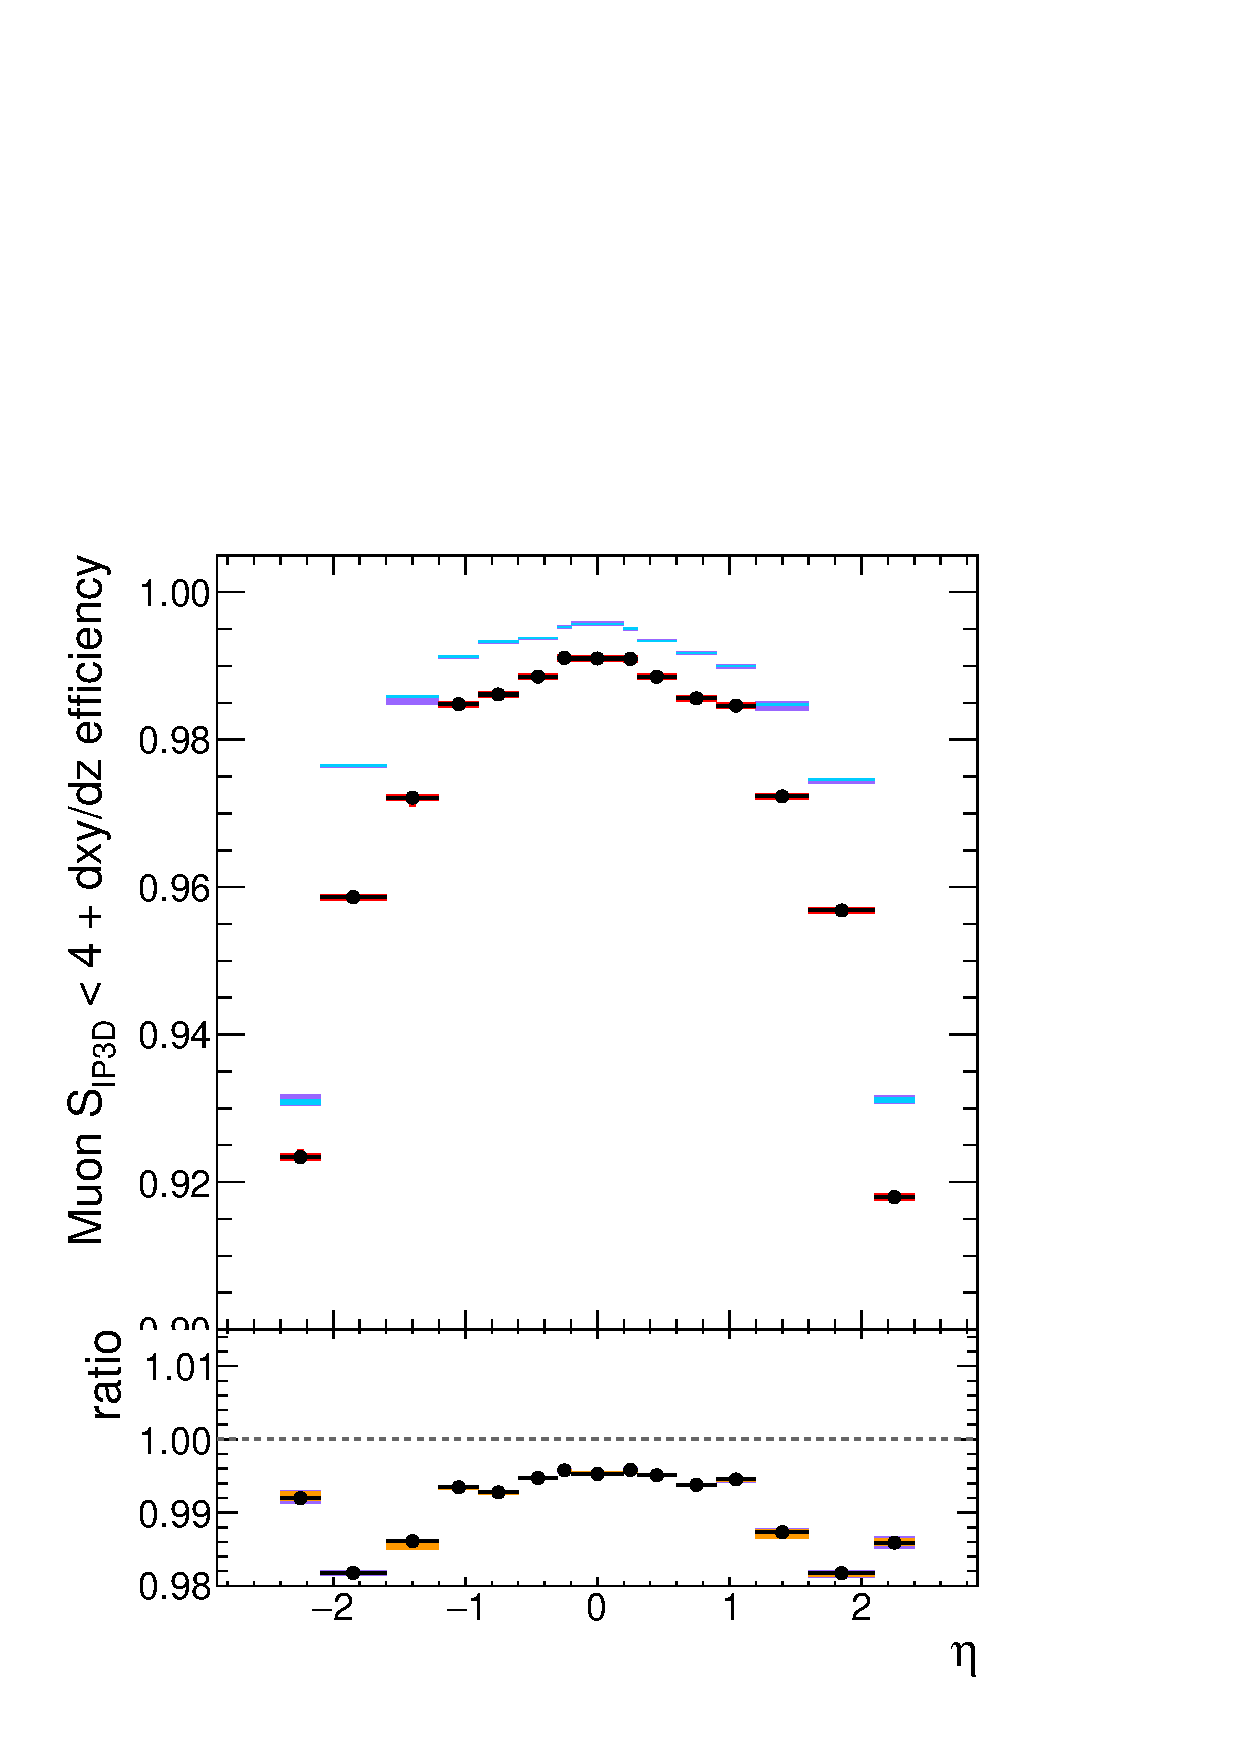
\includegraphics[width=0.32\textwidth]{Figures/Muons/mu_SIP4_pt20.pdf}}
    \caption{Efficiency of the muon impact parameter requirements, measured with the $TnP$ method on $\Z$ events, in bins of \pt in barrel (left) and endcaps (center), and in terms of $\eta$ for all $\pt$ (right). In upper panel, the larger uncertainty bars include also the systematical uncertainties, while the smaller ones are purely statistical. In the lower panel showing the ratio of two efficiencies, black error bars are for statistical uncertainty, the orange rectangles for the systematical uncertainty and the violet rectangles include both uncertainties.}
    \label{fig:MuonIDEff_2}
\end{center}
\end{figure}

\paragraph*{Efficiency measurement of muon isolation requirements}
Isolation efficiency is measured using events from the $\Z$ decay for any \pt. The events are selected with either of \verb=HLT_IsoMu27_v*= or \verb=HLT_Mu50_v*= triggers (for 2017 \verb=HLT_IsoMu27_v*= is used and for 2016 measurements, $OR$  condition is required among \verb=HLT_IsoMu20_v*=, \verb=HLT_IsoTkMu20_v*=, \verb=HLT_IsoMu22_v*=, \verb=HLT_IsoTkMu22_v*=, \verb=HLT_IsoMu24_v*=, \verb=HLT_IsoTkMu24_v*=). 
%\begin{itemize}
%	\item \textbf{2016:}  \verb=HLT_IsoMu20_v*= OR \verb=HLT_IsoTkMu20_v*= \verb=HLT_IsoMu22_v*= OR \verb=HLT_IsoTkMu22_v*= OR \verb=HLT_IsoMu24_v*= OR \verb=HLT_IsoTkMu24_v*=
%	\item \textbf{2017:} \verb=HLT_IsoMu27_v*= 
%\end{itemize}
%}.
The isolation of the muons are calculated after recovery of the FSR photons and subtracting their contribution to the isolation cone of the muons. There are details described of this method which can be found in Ref.~\cite{AN-16-217}.

The results are shown in Figure ~\ref{fig:MuonIDEff_3}.
\begin{figure}[htbp]
  \begin{center}
    \subfigure[]{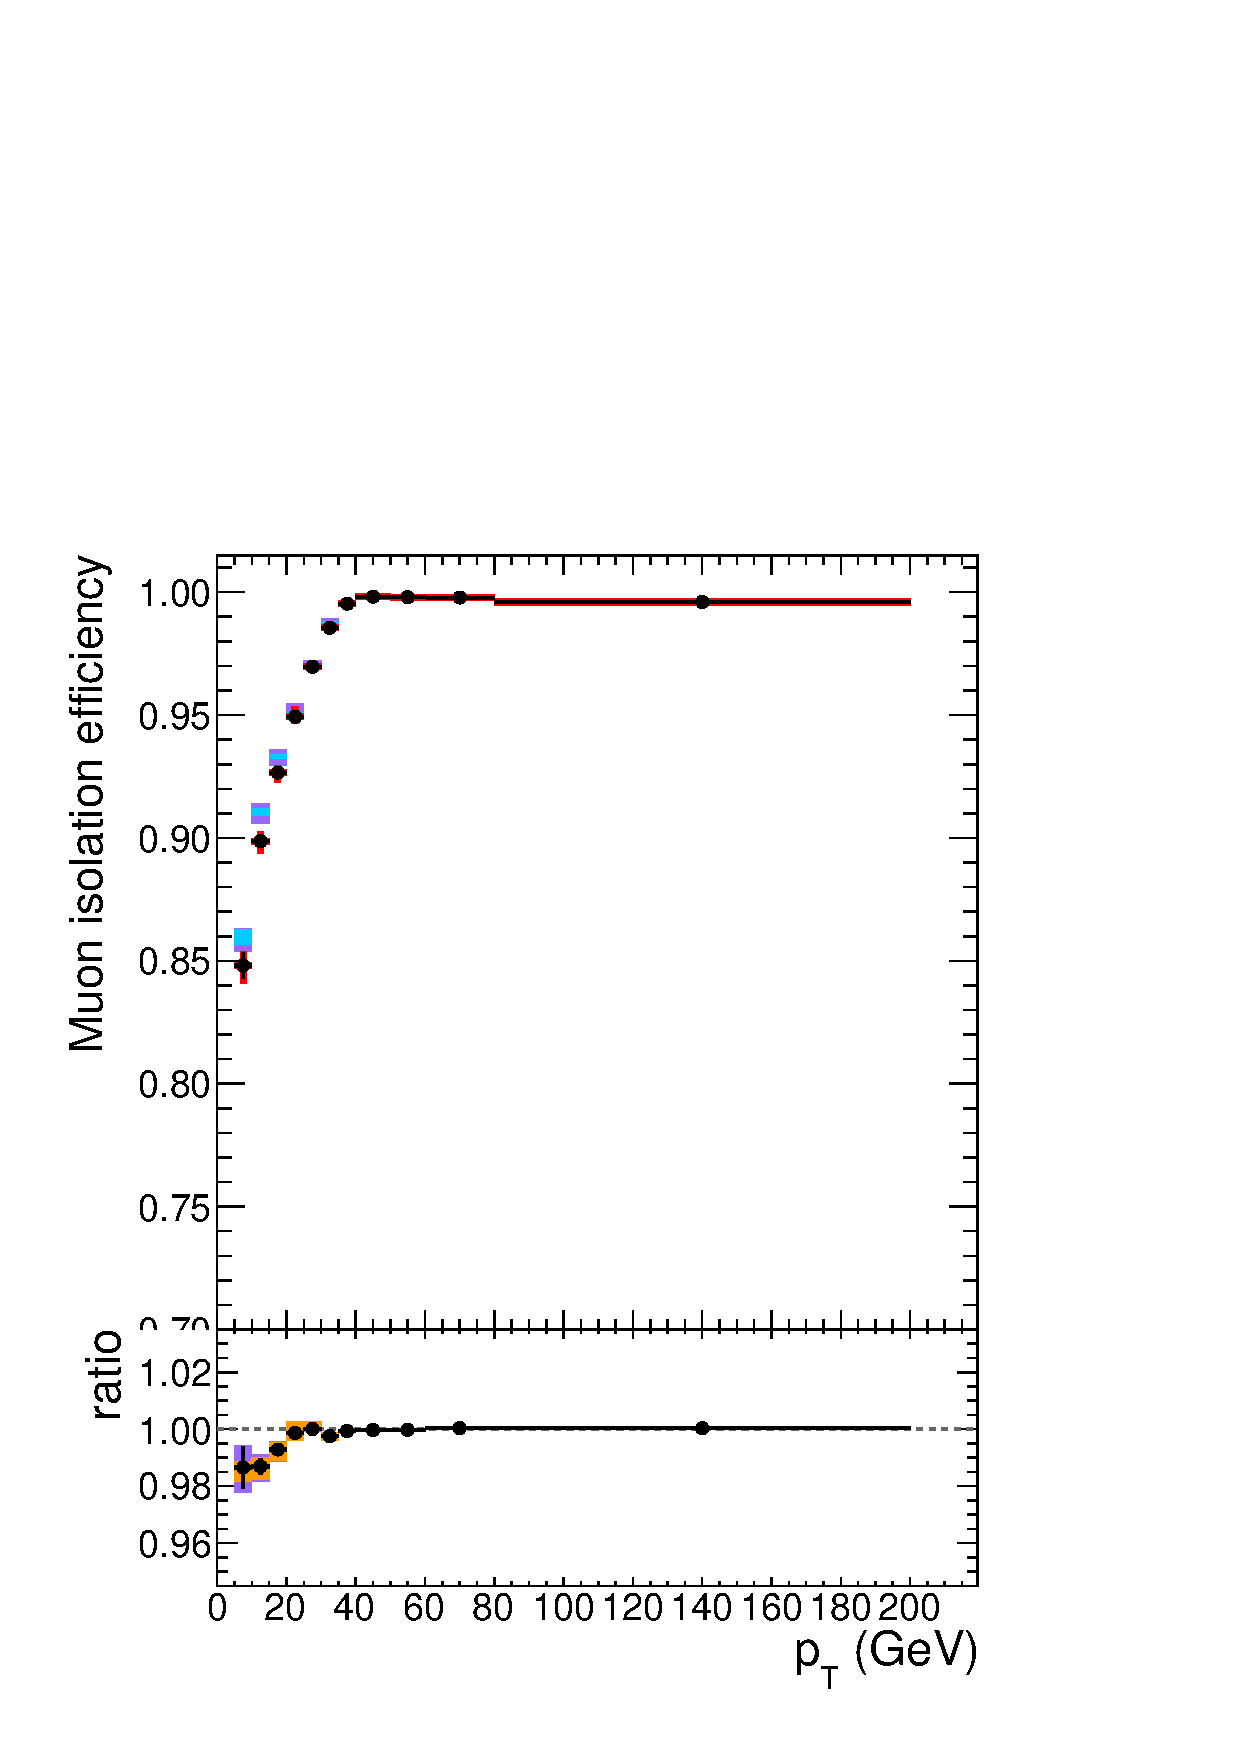
\includegraphics[width=0.32\textwidth]{Figures/Muons/mu_Iso_barrel.pdf}}
    \subfigure[]{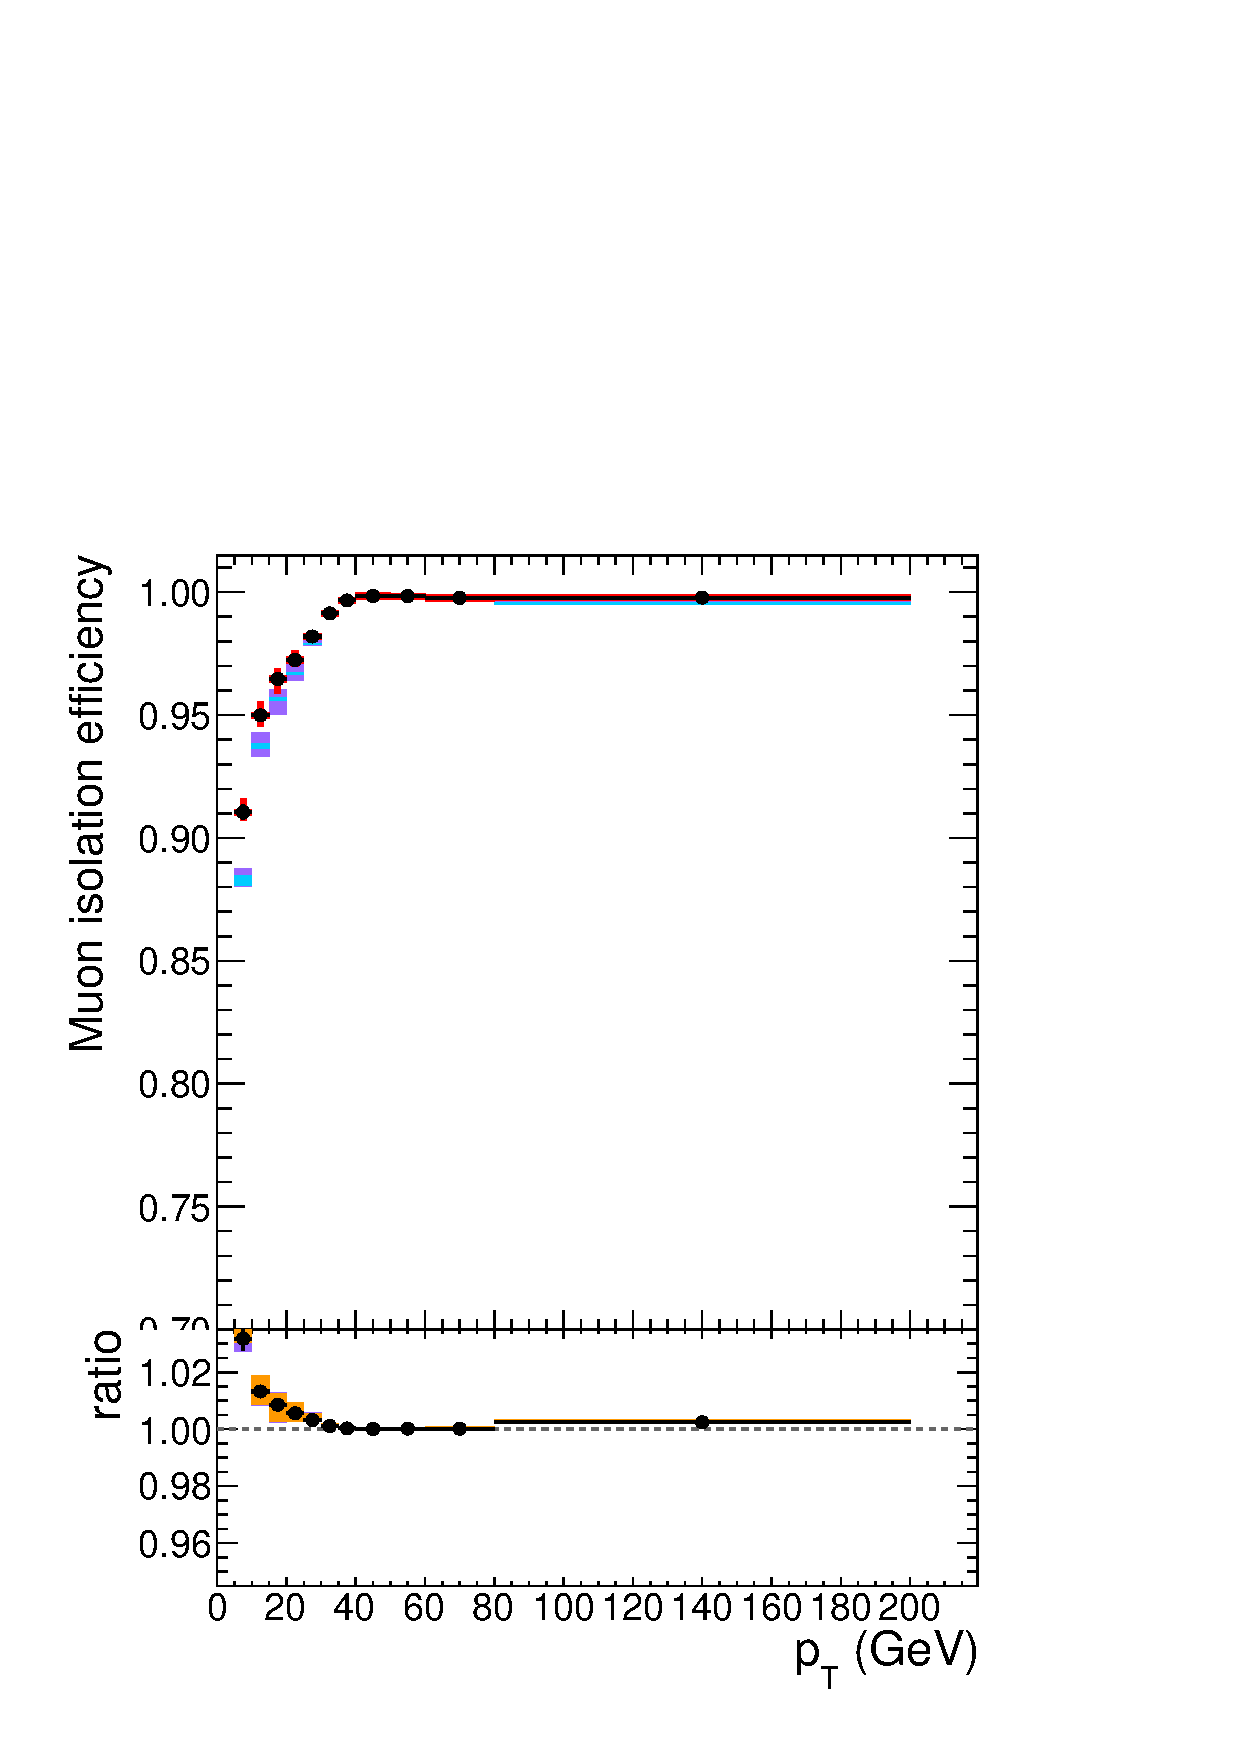
\includegraphics[width=0.32\textwidth]{Figures/Muons/mu_Iso_endcap.pdf}}
    \caption{Efficiency of muon isolation requirement, measured with the tag\&probe method on \Z events, as function of \pt in the barrel (left) and endcaps (right). In the upper panel, the larger error bars include also the systematical uncertainties, while the smaller ones are purely statistical. In the lower panel showing the ratio of the two efficiencies, the black error bars are for the statistical uncertainty, the orange rectangles for the systematical uncertainty and the violet rectangles include both uncertainties.}
    \label{fig:MuonIDEff_3}
\end{center}
\end{figure}

\paragraph*{Tracking}
Tracking efficiency (i.e. efficiency to associate a track to some muon in inner detector) is almost 100\% as shown in the Figure. \ref{fig:eff_tracking} and hence muon Physics Object Group no more recommends tracking scale factors in the analyses. % measured using as probes tracks 
%The efficiency to reconstruct a muon track in the inner detector is measured using as probes tracks
%reconstructed in the muon system alone. The method for measuring the tracking efficiency is the same as 
% in Ref.~\cite{CMS_AN_2015-215}, and the results on 2018 data are briefly discussed here. The efficiency and 
%data to mc scale factors are measured from Z events as a function of $\eta$ for $\pt > 10\GeV$ and $\pt < 10\GeV$. The values of data to mc scale factors 
%used are from the ReReco version of the full dataset collected in 2018. 

%The tracking efficiency in data and simulation as a function of $\eta$ is shown in Fig.~\ref{fig:MuonIDEff_4}.
%\begin{figure}[htbp]
%  \begin{center}
%    \subfigure[]{
\includegraphics[width=0.42\textwidth]{Figures/Muons/Placeholder.png}}
%    \subfigure[]{
\includegraphics[width=0.42\textwidth]{Figures/Muons/Placeholder.png}}
%    \caption{Tracking efficiency in data and simulation as a function of $\eta$ for muon $\pt < 10\GeV$(left) and $\pt > 10\GeV$(right) with ReReco data.}
%    \label{fig:MuonIDEff_4}
%\end{center}
%\end{figure}

\paragraph*{Overall results of muon Scale Factors}
The product of all scale factors for reconstruction, identification, impact parameter and isolation requirements is shown in two dimensional display in Figure ~\ref{fig:MuonIDEff_5}. The figure also shows overall uncertainty on scale factors.  
%The overall correction is about $-1\%$ or less for most \pt and $\eta$ values, increasing to about $-2\%$ in for muons below $10\GeV$ or with $|\eta|>2$.
\begin{figure}[htbp]
  \begin{center}
    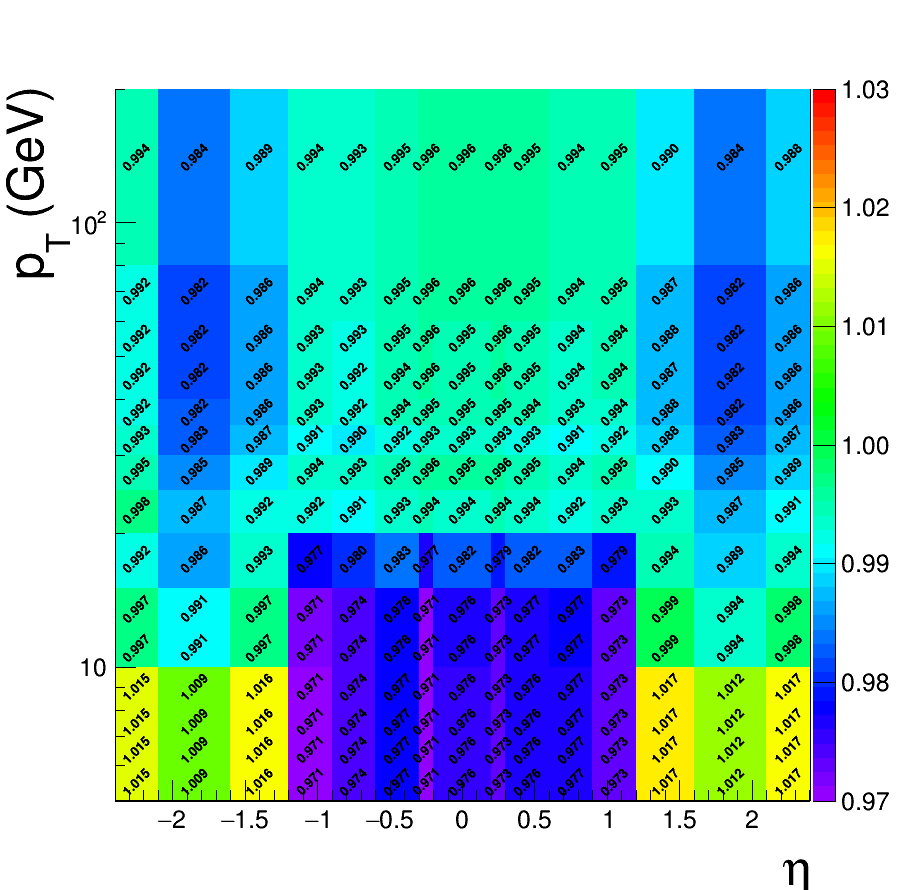
\includegraphics[width=0.45\textwidth]{Figures/Muons/HZZ_SF_2018_RunA2D_2801.png}
    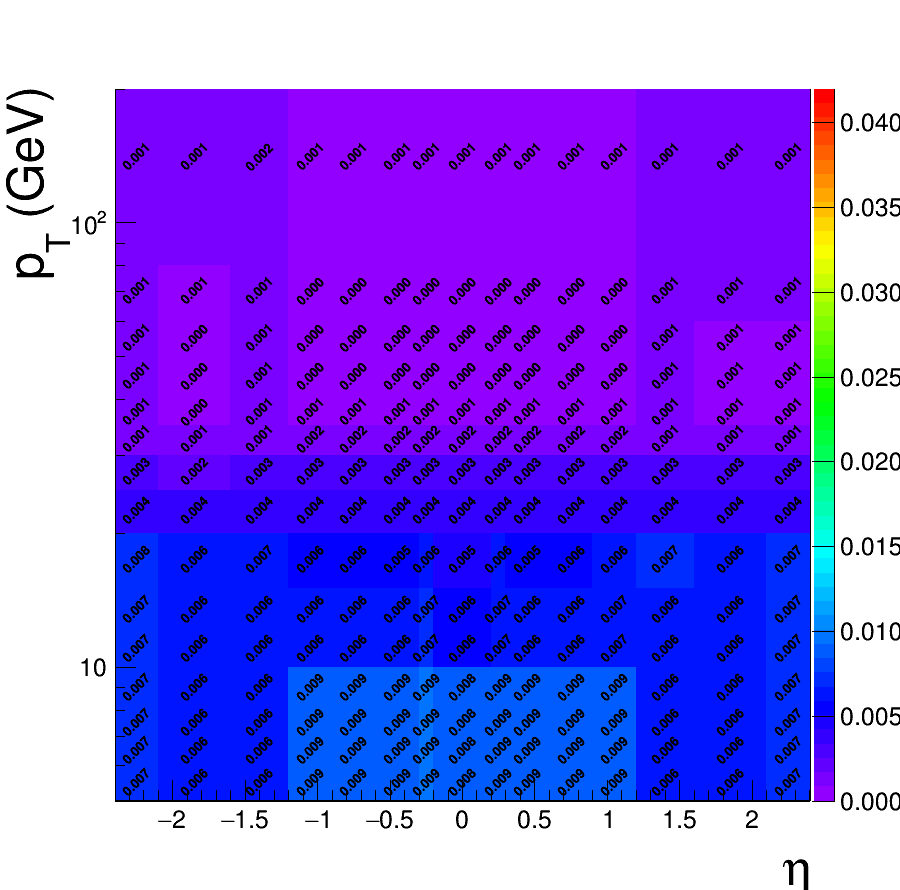
\includegraphics[width=0.45\textwidth]{Figures/Muons/HZZ_SF_errors_2018_RunA2D_2801.png}
    \caption{Left: Overall scale factors for muons, as function of \pt and $\eta$. Right: Uncertainties on overall scale factors  muons shown in two dimensions of \pt and $\eta$.}
    \label{fig:MuonIDEff_5}
\end{center}
\end{figure}

